\documentclass[12pt]{exam}

\usepackage{ge13}
\usepackage{comment}
\usepackage{graphicx}
\usepackage{hyperref}
\urlstyle{rm}   % change fonts for url's (from Chad Jones)
\hypersetup{
    colorlinks=true,        % kills boxes
    allcolors=blue,
    pdfsubject={NYU Stern course GB 2303, Global Economy},
    pdfauthor={Dave Backus @ NYU},
    pdfstartview={FitH},
    pdfpagemode={UseNone},
%    pdfnewwindow=true,      % links in new window
%    linkcolor=blue,         % color of internal links
%    citecolor=blue,         % color of links to bibliography
%    filecolor=blue,         % color of file links
%    urlcolor=blue           % color of external links
% see:  http://www.tug.org/applications/hyperref/manual.html
}

% for ge05.sty
\def\ClassName{The Global Economy}
%\def\Category{Professor David Backus}
\def\Category{Backus \& Cooley}
\def\HeadName{Problem Set \#1}
\newcommand{\phm}{\phantom{--}}
\newcommand{\NX}{\mbox{\it NX\/}}

\printanswers

\begin{document}
\parindent = 0.0in
\parskip = \bigskipamount
\thispagestyle{empty}%
\Head

\centerline{\large \bf \HeadName: Macroeconomic Data}
\centerline{Revised:  \today}

\medskip
{\it You may do this assignment in a group.
Whatever you hand in should be the work of your group
and include the names of all of the contributors.}

\begin{questions}

%\begin{solution}
%Brief answers follow,
%but see also the spreadsheet posted on the course website.
%\end{solution}

% --------------------------------------------------------------------
\question National accounts in Margaritaville (40 points).
Jimmy Buffett has decided to apply for membership in the European Union
on behalf of his newly sovereign nation, Margaritaville.
As part of his application, he must provide the EU
technocrats with a complete set of national accounts.
You have been hired as the Chief National Accountant.
Your first day on the job,
you receive an official Coral Reefer Crew{\texttrademark} t-shirt
and the following information about local economic activity:
%
\begin{itemize}
\item Local Cheeseburger in Paradise{\texttrademark} cafes
sold \$55,000 worth of cheeseburgers to local consumers.
Their expenses were:  imported beef and sesame seeds (\$10,000),
locally produced catsup (\$10,000),
wages and benefits (\$22,000), and rent (\$3,000).
Hint: you will need to compute the profit earned by the cafes.

\item Local tomato growers sold \$8,000 worth of tomatoes to domestic
catsup producers and exported another \$3,000 to the US.
They paid land rent (\$1,000) and wages (\$9,000).

\item Local producers of the Margaritaville Frozen Concoction Maker{\texttrademark }
sold \\ \$100,000 worth of blenders;
40\% were exported to Europe, the remainder to local consumers.
Their expenses were \$15,000 worth of imported metal,
\$15,000 for a new CNC machine imported from Germany,
and \$70,000 in wages.

\item The domestic catsup industry sold \$10,000 worth of product to local
cafes.
They purchased \$8,000 worth of tomatoes from domestic growers
and paid \$2,000 in wages.


\item The newly-formed government collected \$10,000 in taxes from its citizens
and paid \$10,000 to government regulators, who oversee food and beverage safety.
\end{itemize}
%
You mission is to use this raw data to construct
national income and product accounts for Magaritaville.
Specifically:
%
\begin{parts}
\part Compute the value-added of each production unit.
What is GDP?
(10~points)

\part Compute GDP and its expenditure components (consumption,
investment, government purchases of goods and services,
exports, and imports).
(10~points)

\part What are saving and investment?  Why are they different?
Where does the difference go?
(10~points)

\part Jimmy looks over your calculation in (a) and is worried
that you made a mistake.
Over a couple Land Shark Lagers{\texttrademark}
you explain to him that GDP can be computed three different ways:
the sum of value-added across production units (Gross Domestic Product),
the sum of expenditure components (Gross Domestic Expenditure),
and the sum of payments to labor and capital (Gross Domestic Income).
You do the remaining one, payments to labor and capital,
and show him that you get the same answer.
He buys you a margarita to show his appreciation.
(10~points)
\end{parts}

\begin{solution}
It's easiest to do the whole thing on a spreadsheet --- see the link on
the course website.
The idea is to calculate value added, income, and final sales,
as we did in class.
It includes government production,
which is valued at cost (income = value added),
investment,
which is not counted as an expense,
and imports.

\begin{parts}
\part Here's a quick overview of value added by producer:
\begin{itemize}
\item Cafes:  Value added comes from
sales of 55 minus intermediate goods of 20,
which gives you value-added of 35.
On the income side this corresponds to 22 to labor, 3 in rent, and 10 of profit
to the owner.
\item Tomatoes:  Value added is 11, which equals
income of 11 (9 to labor, 1 to rent, 1 of profit).
\item MFCM:  Value added is sales of 100 minus the 15 of metal,
for a total of 85.
By convention, we do not include the 15 of new machines as an expense,
because it's an investment in new plant and equipment.
On the income side, that consists of wages of 70 and profit of 15.
\item Catsup:  Revenue of 10 minus intermediate inputs of 8
gives us value-added of 2, which is paid as wages.
\item Government.  Wages of 10 count (by convention) as value added of 10,
all of it income to government workers.
\end{itemize}
Adding it all up gives us GDP of 143.

\part Expenditures are
\begin{itemize}
\item Cafes:  All of the sales revenue is final sales to consumers.
How do we handle the input of imported beef and seeds?
One approach is to put a 10 in imports, which therefore makes a negative
contribution to expenditures on (our) GDP.
The approach we follow in the spreadsheet is to introduce
and extra production unit which sells beef and seeds to us.
They give us the same answer.
\item Tomatoes:  Only the exports of 3 counts as final sales,
the rest is an input to the catsup producer.
\item MFCM:
Finals sales includes consumption of 60, exports of 40, imports of 30,
and investment of 15.
The investment really goes with the foreign machine producer,
which is how it's listed in the spreadsheet:  an investment of 15
and an import of 15.
As with the seed producer, we note this with a separate column.
\item Catsup:  None of it counts as final sales, since it's sold to cafes
and used by them as an intermediate product (an input).
\item Government.  Government purchases are 10:
by convention, it ``purchases'' what it produces.
\end{itemize}
Adding it all up gives us the expenditure identity:
\begin{eqnarray*}
    Y (\mbox{GDP} = 143) &=& C (115) + I (15) + G (10) + \NX (43-40) .
\end{eqnarray*}
\part From above, $S = Y - C - G = 18$ and $I = 15$.
Net exports $\NX = 3$ accounts for the difference:  $ S = I + \NX$.
In this case, it means we are contributing 3 to foreign capital markets:
domestic saving is more than we need to finance domestic investment,
so we send the rest abroad.
\part Value added by production unit, in the order they appear in the question:
\begin{eqnarray*}
        \mbox{Value added}  &=& 35 + 11 + 85 + 2 + 10 \;\;=\;\; 143 .
\end{eqnarray*}
The only one we're missing is income, which (of course)
is the same as value added.
Summing again across production
units in order of appearance:
\begin{eqnarray*}
       \mbox{Gross Domestic Income} &=&  35 + 11 + 85 + 2 + 10 \;\;=\;\; 143 .
\end{eqnarray*}
Thus we have three ways to get the same number:  value added, income,
and expenditures.
The numbers are all the same, so we can drink our margarita in peace.


\end{parts}
\end{solution}

%\begin{comment}
% --------------------------------------------------------------------
\question Inputs and outputs (20 points).
Specify the most likely direct impact of each of the following
on the components of the production function.
Don't make this more complicated than it is:
we're concerned here only with
the impact on the components of the production function.
%
\begin{parts}
\part A new office building in Wuhan, China.  (5~points)
\part A reduction in the minimum wage that leads more people to work. (5~points)
\part A more efficient air-conditioning system to replace the old one
in the Kaufman Management Center. (5~points)
\part A reduction in tariffs in Brazil on imported computer equipment. (5~points)
\end{parts}

\begin{solution}
You may recall that the production function links output $Y$
to inputs of capital $K$ and labor $L$ and productivity $A$:
\begin{eqnarray*}
    Y &=& A K^{1/3} L^{2/3} .
\end{eqnarray*}
\begin{parts}
\part An increase in capital, which should raise output, too.
\part An increase in labor, which should raise output.
\part If it's more efficient, then it will produce the same output
with less energy use, so it's an increase in productivity,
which should raise output.
And it could raise productivity in other ways, too ---
say, we're more comfortable so we work harder.
\part This makes computer equipment cheaper, which should increase the capital
stock and thus output.
It could also raise productivity
by giving Brazilian firms cheaper/better access to the best computer technology.

From a paper by Cole, Ohanian, Riascos, and Schmitz (``Latin America
in the rearview mirror'') (rough paraphrase):
\begin{quote}
In 1977, Brazil embarked on a zero-quota policy that
meant that only PCs and minicomputers produced by Brazilian-owned firms
could be sold in Brazil.
Moreover, the black market was not a practical choice for large firms.
The policy insulated Brazilian computer producers from foreign competition
and featured entry barriers to new Brazilian producers through
a maze of bureaucratic requirements.

When the quota was lifted by President Collor in 1992,
productivity in Brazil�s computer industry rose dramatically
and 6 of the top 10 firms selling in Brazil in the mid-1990s were
Brazilian.
Productivity of computer users also increased,
as firms got access to better equipment at lower prices.
\end{quote}

\end{parts}
\end{solution}

% --------------------------------------------------------------------
\question Investment and saving in China (40~points).
China is well known for its unusually high saving and investment rates.
Our mission here is to document both for the period since 1980.

We'll use the data in the spreadsheet linked to the course outline
and posted at

\vspace*{\parskip}
\centerline{\url{http://pages.stern.nyu.edu/~dbackus/2303/ps1_q3_s13.xls}}

The first sheet, {\tt Data for Q3}, includes everything you need:
GDP and its expenditure components at current prices.
The second, {\tt OECD source data}, is the data exactly as it comes
from the OECD's Annual National Accounts database.
It includes more categories and uses official data descriptions,
which can be mysterious if you haven't seen them before.

\begin{parts}
\part Is ``GDP at current prices'' ``real'' or ``nominal''?
What does that mean anyway?
(10~points)

\part Check the expenditure identity, $ Y = C + I + G + \NX$.
Why isn't it satisfied here?
(10~points)

\part Graph saving, investment, and net exports as ratios to GDP.
As in class, we define saving as $S = Y - C - G $.
(10~points)

\item Looking at your figure,
how important are foreign sources of funds to Chinese investment?
How can you tell?
(10~points)
\end{parts}



\begin{solution}
\begin{parts}
\part When we measure something ``at current prices''
we say it's a nominal magnitude, measured in units of money.
When we measure something instead ``at constant prices,''
we say it's a real magnitude.
All of the variation over time is in the quantities,
because we're using the same prices at all dates.
So real GDP measures the quantity of goods and services produced
and nominal GDP measures their value (prices times quantity)
in units of currency.

\part The expenditure identity doesn't quite work in this case,
which means the data are internally inconsistent.
The inconsistency is captured by a statistical discrepancy in this case,
an official admission of the problem.

\part Here's the graph:
\begin{center}
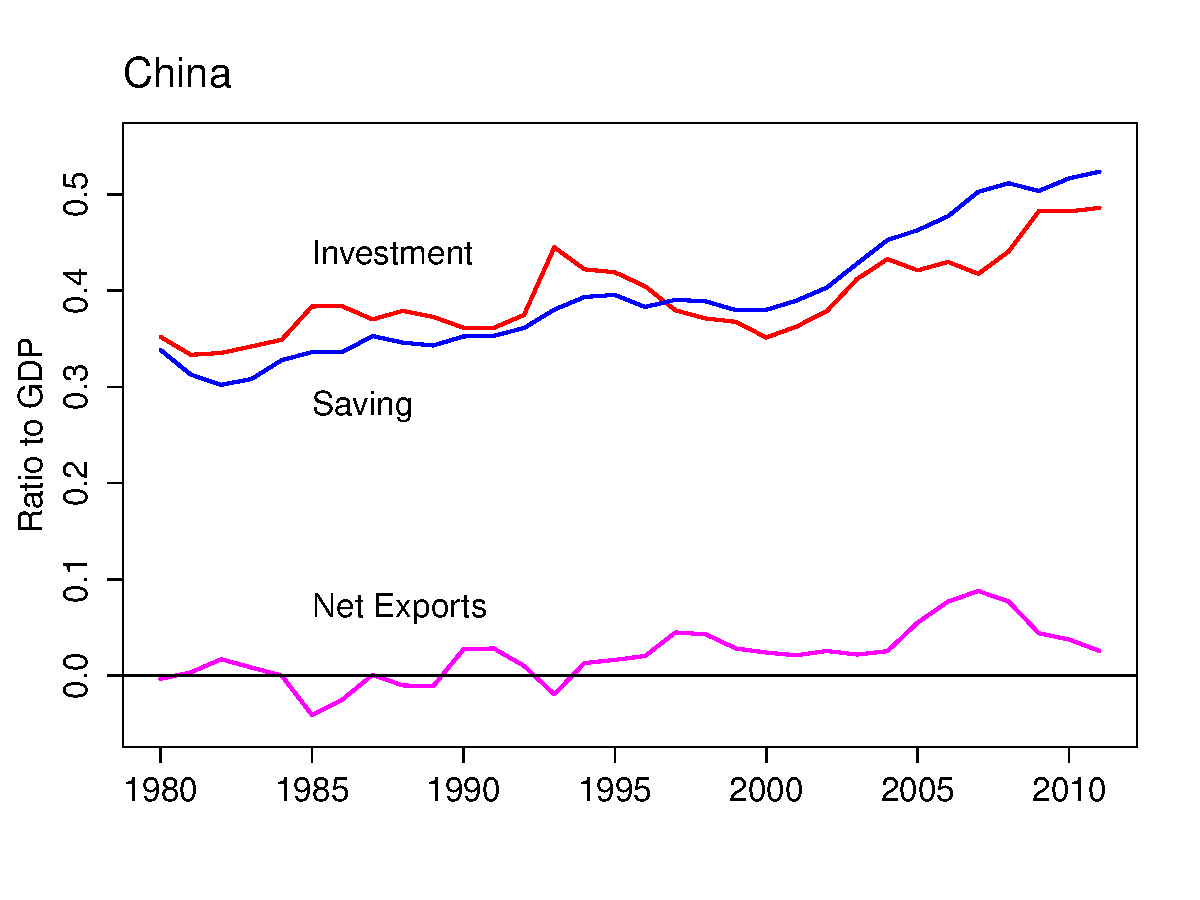
\includegraphics[scale=0.5]{China_shares.pdf}
\end{center}
%
We're simply reminding ourselves of the connection
between GDP and various combinations of expenditures.
Specifically, in the notation we've used before:
\begin{eqnarray*}
        S &=& Y - C - G \;\;=\;\; I + \NX .
\end{eqnarray*}

\part The point here is that net exports reflects international
movements of capital.
If $\NX > 0$, as it has been recently, then we have more saving
than investment, and the extra funds are invested abroad as
a ``capital outflow.''
That's the source of the ``China is buying the US'' talk you hear.
Since capital is flowing out, foreign capital plays little role
on average in financing Chinese investment.
In fact, you can see from the figure that international capital flows
(net exports) are small relative to both saving and investment.
\end{parts}
\end{solution}

\end{questions}

\vfill \centerline{\it \copyright \ \number\year \
NYU Stern School of Business}

\end{document}

